\begin{mdframed}[style=warning]
	\begin{ejercicio}
		Demuestre que el camino seguido por un oscilador isotrópico en dos dimensiones, para $\alpha - \beta = \pm \flatfrac{\pi}{2}$, es una elipse.\\
		\textit{Hint: Reescriba $y(t) = A_y \sin{\qty(\omega t - \alpha + (\alpha - \beta))}$.}
	\end{ejercicio}
\end{mdframed}



\begin{mdframed}[style=warning]
	\begin{ejercicio}
		Considere un oscilador anisotrópico en dos dimensiones.
		\begin{enumerate}
			\item Demuestre que si la razón entre las frecuencias $\frac{\omega _x}{\omega _y}$ es un número racional entonces el movimiento es periódico.
			\item Demuestre que si la razón entre las frecuencias $\frac{\omega _x}{\omega _y}$ es un número irracional entonces el movimiento nunca se repite.
		\end{enumerate}
	\end{ejercicio}
\end{mdframed}



\begin{mdframed}[style=warning]
	\begin{ejercicio}
		Encuentre el periodo de oscilacion de una esfera sólida de masa $M$ y radio $R$ respecto a un punto en su superficie.
	\end{ejercicio}
\end{mdframed}



\begin{mdframed}[style=warning]
	\begin{ejercicio}
		Un bote esta flotando en un gran contenedor de agua como se ve en la figura \ref{ej4}. El bote está en equilibrio sumergido una distancia $d_o$. Demuestre que si es empujado a una distancia $d$ y se suelta, se inducirá un movimiento armónico. Encuentre su frecuencia de oscilación. Si $d_o = 20cm$, cual es el periodo?
		
		\begin{figure}[H]
			\centering
			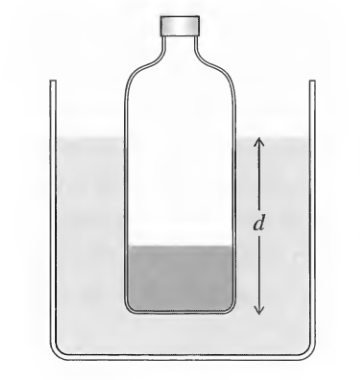
\includegraphics[scale=0.3]{./img/ej4.png}
			\caption{\centering El bote tiene arena para que pueda flotar verticalmente. Esta en equilibrio a una profundidad de $d_o$.}
			\label{ej4}
		\end{figure}
	\end{ejercicio}
\end{mdframed}



\begin{mdframed}[style=warning]
	\begin{ejercicio}
		Considere un oscilador armónico simple con peroido $\tau$. Sea $\expval{f}$ el valor promedio de cualquier variable $f(t)$, promediado durante un ciclo completo:
			$$ \expval{f} = \frac{1}{\tau} \int _0 ^\tau f(t) \dd{t}. $$
		Pruebe que $\expval{T} = \expval{V} = \frac{1}{2} E$ donde $E$ es la energía total del oscilador.
	\end{ejercicio}
\end{mdframed}

\textbf{Reto:}

\begin{mdframed}[style=warning]
	La masa mostrada en la figura \ref{reto} esta en reposo en una mesa sin fricción. Cada uno de los dos resortes identicos con costante $k$ y longitud natural $l_o$. El punto de equilibrio está en el origen, y la distancia $a$ no necesariamente igual a $l_o$. Demuestre que cuando la masa se mueve a una posición $(x,y)$, con $x$ y $y$ pequeños, la energía potencial tiene la siguiente forma
		$$ V(x,y) = \frac{1}{2} k_x x^2 + \frac{1}{2} k_y y^2, $$
	para un oscilador anisotrópico. También demuestre que si $a < l_o$ el punto de equilibrio del origen es inestable.
	\begin{figure}[H]
		\centering
		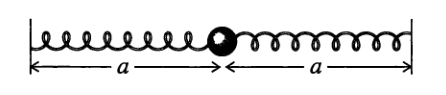
\includegraphics[scale=0.5]{./img/reto.png}
		\caption{Problema reto.}
		\label{reto}
	\end{figure}
\end{mdframed}





















%%

